\section{Unity Features}

\subsection{NavMeshes}

Um die zu erlernenden Aufgaben zu vereinfachen, bietet es sich an, Wegfindungsalgorithmen zu nutzen (siehe Abschnitt \ref{subsubsec:agentnavmesh}). Unity bietet daf"ur das sogenannte \texttt{NavMesh} an.
\\
Ein \texttt{NavMesh} stellt die begehbare Fläche der Szene dar. Ein Agent, welcher sich auf dem NavMesh befinden, kann eine Anfrage mit einem gew"unschten Zielpunkt an das \texttt{NavMesh} senden. Das \texttt{NavMesh} generiert dann eine Liste an Punkten auf dem \texttt{NavMesh}. Von einem Punkt am Index $i$ zu einem Punkt $i+1$ existiert dabei immer eine gerader Weg ohne Hindernisse. Außerdem existiert ein gerader Weg von der Position des Agenten zum Zeitpunkt der Generierung des Pfades zum Punkt am Index $0$. Der letzte Punkt des Pfades ist nat"urlich der gew"unschte Zielpunkt.
\begin{figure}
	\centering
	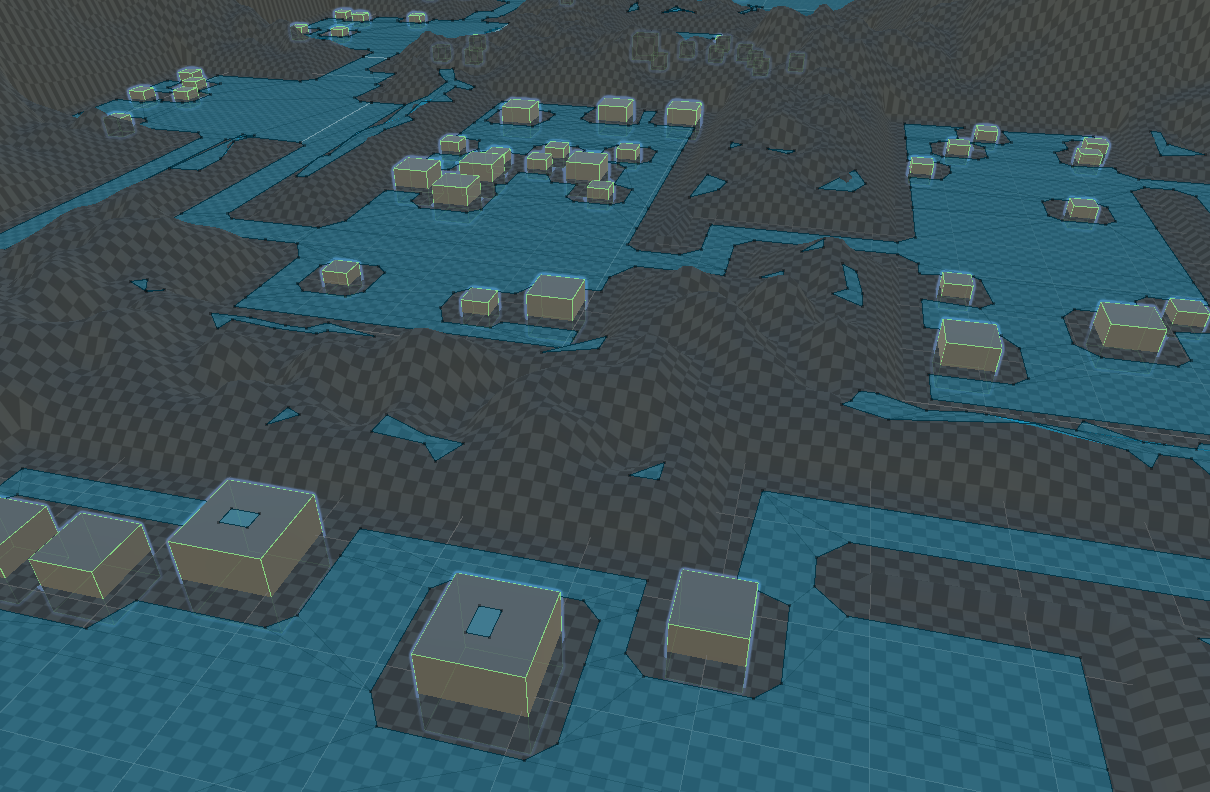
\includegraphics[width=0.8\linewidth]{resources/img/navMesh01.png}
	\caption{Prozedual generierte Umgebung mit \texttt{NavMesh} (in blau)}
	\label{fig:navMesh01}
\end{figure}
\\
Es gibt diverse M"oglichkeiten, ein \texttt{NavMesh} in Unity benutzen. Wir haben uns dazu entschieden, unserem \texttt{Terrain}-Objekt die Komponente \texttt{NavMeshSurface} zu geben.
\\
Zu Beginn m"ussen wir der Komponente einige Informationen "uber unseren Agent mitteilen. Diese Informationen umfassen:
\begin{itemize}
	\item Den \textit{Agent Radius}, um den minimalen Abstand zu Hindernissen bestimmen zu können. Sollte dieser Wert zu groß gew"ahlt sein, kann es unter Umständen passieren, dass der Agent durch engen Passagen nicht durchlaufen kann, obwohl dieser eigentlich klein genug daf"ur wäre.
	\item Die \textit{Agent Height}
	\item Die \textit{Max Slope}, welche die maximale Steigung, die der Agent bewältigen kann, beschreibt.
	\item Die \textit{Step Height}, welche den maximalen H"ohenunterschied mit beliebiger Steigung beschreibt, die der Agent unanhängig von der angegebenen \textit{Max Slope} bewältigen kann. Dies ist dazu notwendig, damit der Agent zum Beispiel eine Treppe hochlaufen kann, da die einzelnen Treppenstufen meistens eine Steigung von $90\deg$ besitzen.
\end{itemize}

\begin{figure}
	\centering
	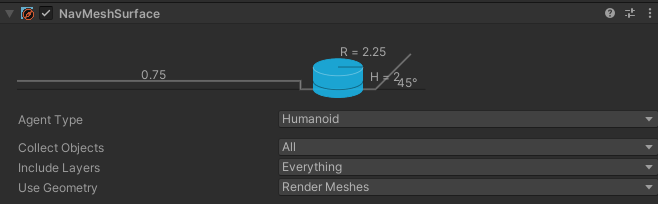
\includegraphics[width=0.8\linewidth]{resources/img/navMesh02.png}
	\caption{Auszug aus den Einstellungen f"ur die \texttt{NavMeshSurface}-Komponente.}
	\label{fig:navMesh02}
\end{figure}

Im nächsten Schritt sammelt das Skript sämtliche geometrischen \texttt{GameObjects} der Szene, um zusammen mit den Informationen "uber den Agent die begehbare Fläche zu approximieren (auch \textit{Baking} genannt).
\\
Ein \texttt{NavMesh} lässt sich auch gut während der Laufzeit des Programmes generieren. In unserem Anwendungsfall ist dies essentiell, da wir die Umgebung "uberhaupt erst zur Laufzeit prozedual erstellen. Eine Vorabgenerierung des \texttt{NavMeshes} wäre daher unmöglich.
